\section{System}
\label{sec:sys}

A \ql query is rewritten into a sequence of algebraic operators, a
particular execution method is selected for each operator, and the
query is executed.  All language operators are also available through
the public API of the \ql library, and may be used like any other
library in an Apache Spark application.

The order of operators within a \ql statement is determined at
execution time, based on a combination of rule-based and cost-based
considerations.  Further, we implement a variety of \tg
representations and partitioning strategies.  Which representation and
which partitioning strategies are used is determined by a combination
of rule-based and cost-based considerations.

{\bf Data representation.}  We developed several different in-memory
representations for the evolving graph to explore the tradeoffs of
compactness, parallelism, and support of different query operators.
The data structures represent a continuum of replication, from the
SnapshotGraph to OneGraph and are described here in more detail.

The simplest way to represent an evolving graph is by representing
each snapshot individually, a direct translation of our logical data
model.  We call this data structure SnapshotGraph and an example is
depicted in Figure~\ref{fig:sgp}.  While this representation is
simple, it is obviously not compact, considering that in most
real-world evolving graphs there is a 99\% simmilarity between
consecutive snapshots~\cite{?}.  In a distributed architecture like
Spark, however, this data structure provides some benefits as it can
be easily parallelized by assigning different snapshots to different
workers with improved temporal locality for snapshot-based analytics.
SnapshotGraph edges can be partitioned using temporal or structural
criteria.  Furthermore, due to Spark's lazy evaluation, operations
such as TSelect are very efficient, since only those snapshots
involved in the operation are loaded.  While other data structures do
not benefit from this feature, push selection in query optimization
can compensate equally well.

\begin{figure}[t!]
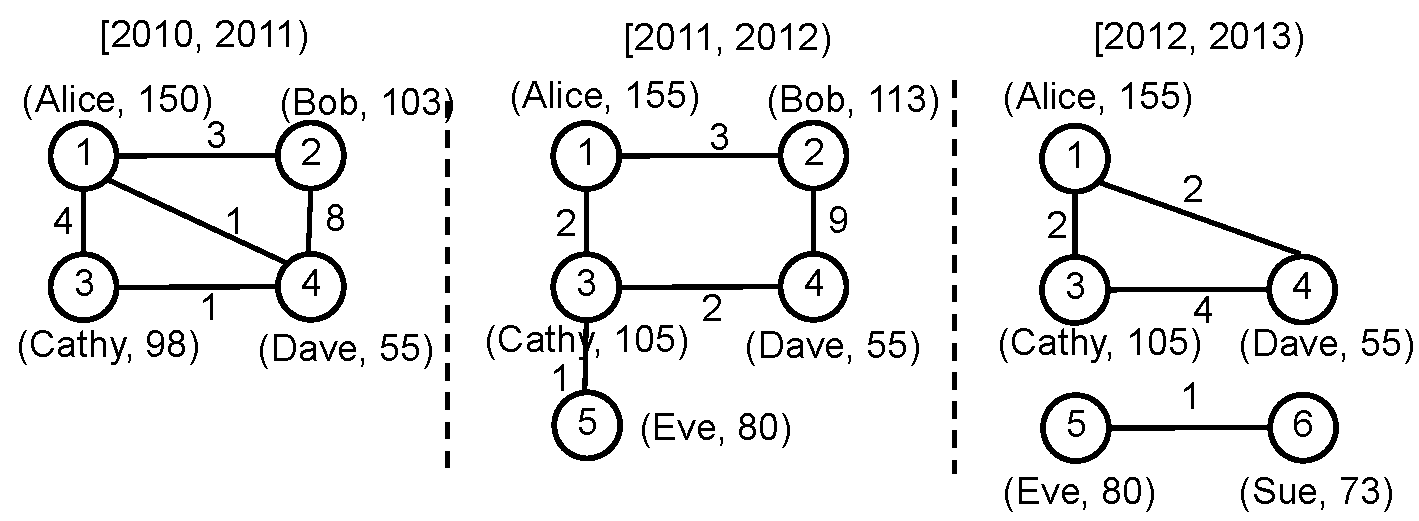
\includegraphics[width=3.2in]{figs/sgp.pdf}
\caption{SnapshotGraph representing T1 from Figure~\ref{fig:tg}}
\label{fig:sgp}
\end{figure}

To take advantage of high similarity between snapshots, we developed
another data structure called MultiGraph (see Figure~\ref{fig:mg}).
MultiGraph stores the evolving graph as a single graph, with one
vertex for all time periods, but one edge per period where it exists.
Because our goal is to represent both topoligical and attribute
information, we need to store not only vertex presence or absence
(which can be easily accomplished by an existence string, like
in~\cite{Kan2009}, or bit sets), but also the values of the vertex
attribute at each time period it existed.  MultiGraph vertex
attribute, thus, is a map of time indices, which are easily converted
to intervals, and corresponding values.  Edge attributes are tuples of
the time index and the value at that time period.  Vertices
historically change less frequently than edges~\cite{?}, so the space
savings on storing each vertex once are about ?? \% in our
experimental data sets.  Some of these savings, however, are taken up
by the storage of a more complex map data structure compared to a
simple single attribute like in the SnapshotGraph.  Partition of the
MultiGraph edges can be either temporal or structural, which lead to
different rates of vertex replication between partitions.

\begin{figure}[t!]
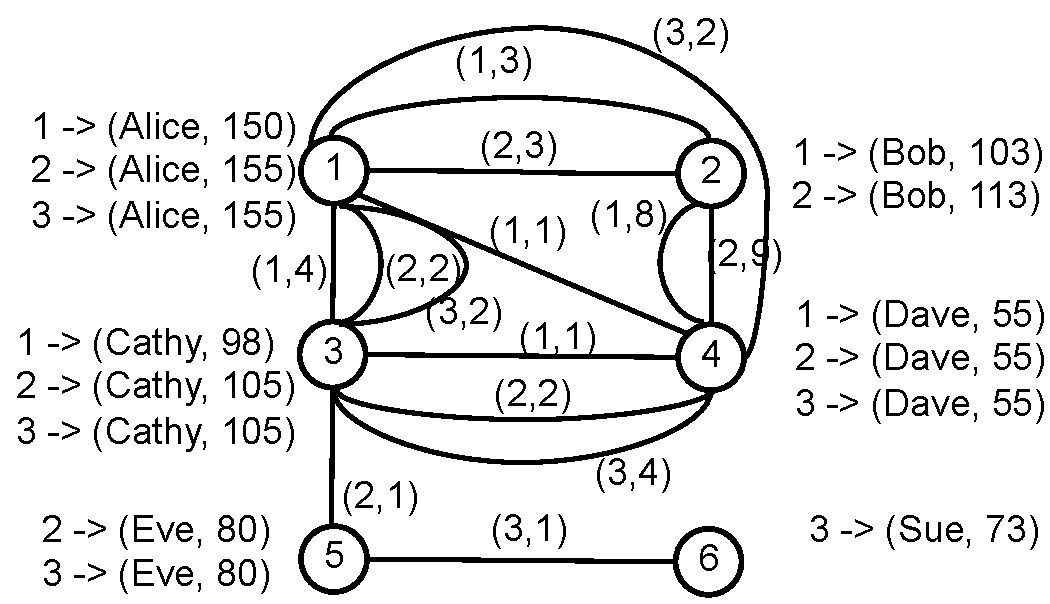
\includegraphics[width=3.2in]{figs/mg.pdf}
\caption{MultiGraph representing T1 from Figure~\ref{fig:tg}}
\label{fig:mg}
\end{figure}

The implementation of some of the Portal operations in MultiGraph is
more complex.  Selection, for example, is a subgraph operation that
operates on all vertices and edges.  TGroup, however, is more
intuitive and benefits from temporal locality.  Implementation of
snapshot analytics like pagerank is done in a batch mode, similar
to~\cite{DBLP:journals/tos/MiaoHLWYZPCC15}.  This data structure
should also be more amenable to cross-time analytics and pattern
mining, which we intend to explore in the future.

Note that for a large subset of queries, the attribute information is
not used, and only the topology is important.  Thus, we can store the
vertex attributes in a separate collection (column store), removing
the attribute map and replacing it with existence bitsets instead.
This is the essence of the MultiGraphColumn data structure, depicted
in Figure~\ref{fig:mgc}.  This kind of representation allows storage
of an arbitrary number of vertex attributes without using complex
per-vertex lists, read from disk only as needed.  Further compression
can be achieved by storing vertex attributes only once across all time
periods where they are the same, similar to how temporal databases
represent this type of data (e.g., see~\cite{Muller2008}).  The
drawback of this approach is that decompression is required to
support, for example, the TGroup operation.

\begin{figure}[t!]
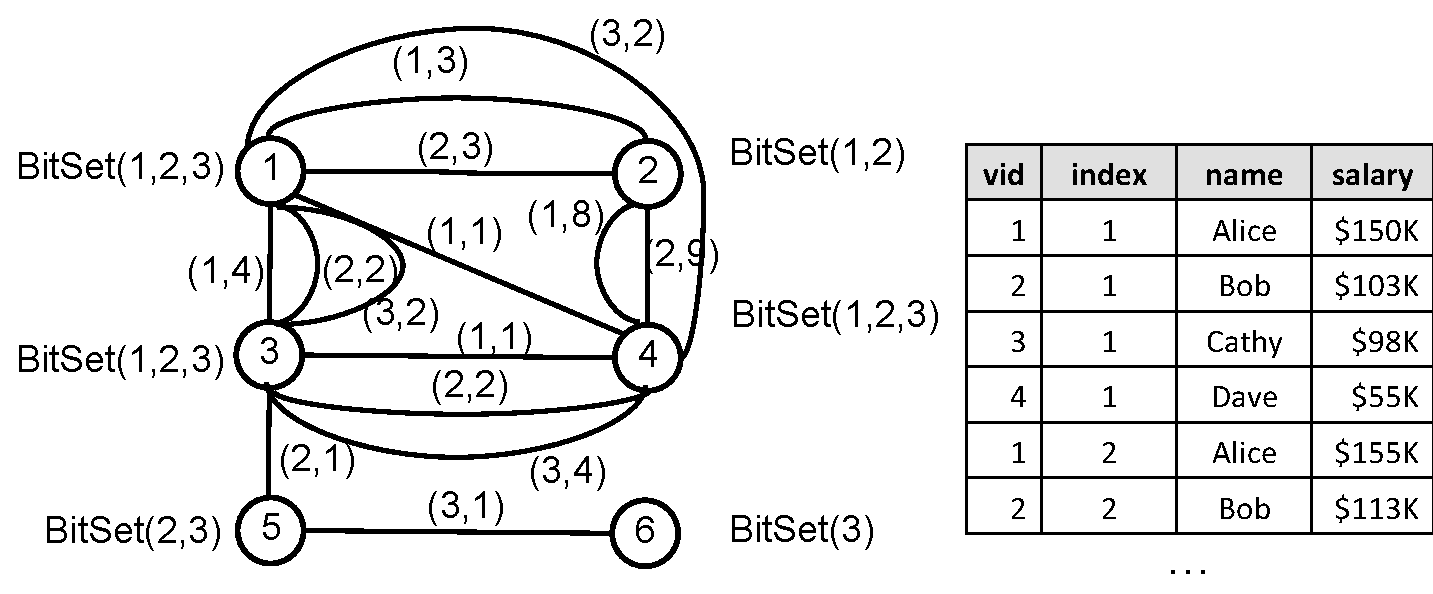
\includegraphics[width=3.2in]{figs/mgc.pdf}
\caption{Column MultiGraph representing T1 from Figure~\ref{fig:tg}}
\label{fig:mgc}
\end{figure}

The most compact, topologically, representation is to store each
vertex {\em and} edge only once for the whole evolving graph, by
taking a union of the snpashot vertex and edge sets.  The OneGraph
data structure uses this representation in our system.  Similar to
MultiGraph, the vertex and edge attributes are stored in maps with
time index - attribute value pairs (see Figure~\ref{fig:og}).
Compared to MultiGraph or SnapshotGraph, this leads to ?? \% storage
savings.  This data structure provides some benefits in addition to
compactness, since it reduces the total communication between vertices
in Pregel-based analytics in batch mode.  The drawback is that
OneGraph cannot be partitioned temporally and is much denser than
individual snapshots (average vertex degree ?? for our nGrams
dataset).

\begin{figure}[t!]
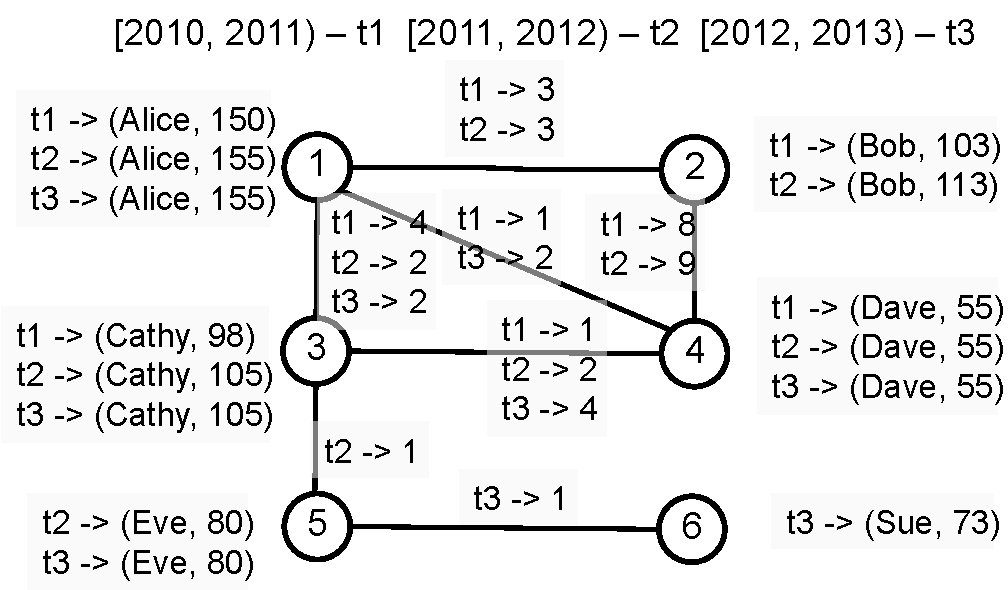
\includegraphics[width=3.2in]{figs/og.pdf}
\caption{OneGraph representing T1 from~\ref{fig:tg}}
\label{fig:og}
\end{figure}

Finally, similar to MultiGraphColumn, OneGraphColumn uses a single
graph to represent the union of vertices and edges, with BitSets for
presence information, while the attribute information is stored
separately.  This is not as compact as storing attributes within the
graph elements, but is faster in many operations where only graph
topology is required.

{\bf Partition Strategies.}  We considered six different edge
partition strategies, which were applied prior to the operation but
after loading:
\begin{enumerate}
\item Canonical Random Vertex Cut (CRVC).  Each edge source and destination
  vertex ids are hashed in a canonical direction, as a tuple, and the
  result is distributed among the available partitions.  The result is
  a random vertex cut that colocates all edges between vertices,
  regardless of direction.  This strategy is available in GraphX and
  was used without modification.
\item 2D Edge Partitioning.  A sparce edge adjacency matrix is
  partitioned in two dimensions.  This guarantees a 2 * sqrt(number of
  partitions) bound on vertex replication and has been shown to be
  highly efficient for structural partitioning~\cite{}.  This strategy
  is also available in GraphX and was used without modification.
\item Naive Temporal.  Provided there are more time intervals in the
  graph than there are partitions, each edge is placed in the time
  index modulo number of partitions place, round-robin fashion.  In
  the case where the graph covers a small time interval, multiple
  partitions are used for each interval (we term this a {\em run}),
  and the CRVC strategy is applied within each run.
\item Consecutive Temporal.  
\end{enumerate}
